%!TEX root = ../../dissertation.tex
%%%%%%%%%%%%%%%%%%%%%%%%%%%%%%%%%%%%%%%%%%%%%%%%%%%%%%%%%%%%%%%%%%%%%%%%%%%%%%%%
\section{Evaluation Methodology}
\label{c4:sec:methodology}

With the mobile network load defined and possible influencing factors described, the findings can now be applied to an actual mobile network. For this data from passive network traces will be employed. But first, the monitoring setup and the captured has to be described in this section. This also includes a description of some methods required to examine specific device types and other device-based factors from the dataset.

While this chapter only employs passive measurements, Chapter~\ref{chap:mobilestreaming-measurements} will additionally deal with approaches to conduct meaningful active device-based measurements and set up a mobile streaming simulation testbed based on some of the results.


%%%%%%%%%%%%%%%%%%%%%%%%%%%%%%%%%%%%%%%%%%%%%%%%%%%%%%%%%%%%%%%%%%%%%%%%%%%%%%%%
\subsection{Network and Monitoring Setup}

For the analysis, the \gls{METAWIN} monitoring system developed in a previous third-party research project and deployed in the network of an Austrian mobile operator is used. Detail information on this setup can be found in \cite{ricciato_2011,ricciato2006traffic}.

\begin{figure}[htb]
	\centering
	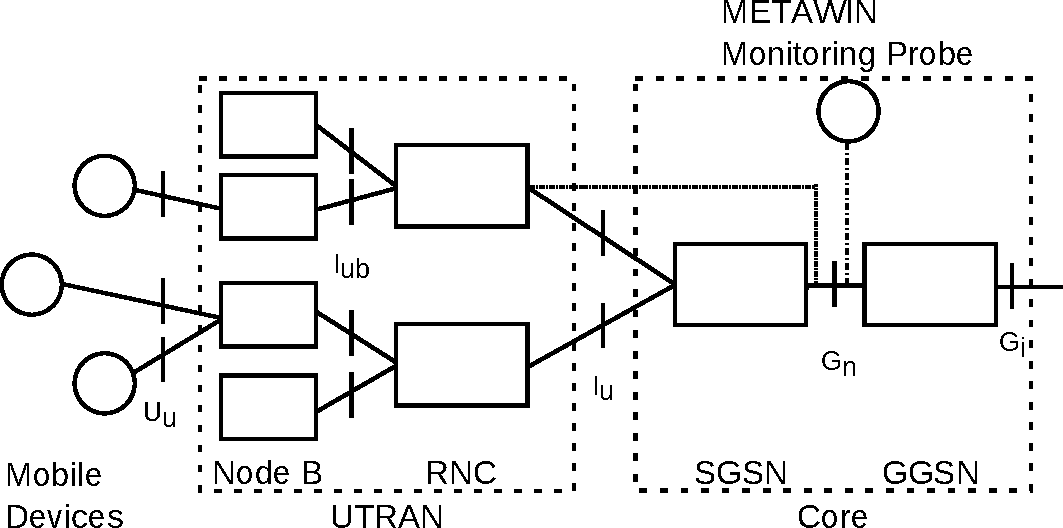
\includegraphics[width=1.0\textwidth]{images/umts-network.pdf}
	\caption{Location of the \acrshort{METAWIN} monitoring probe in the \acrshort{3G} core network.}
\label{c4:fig:umtsnetwork}
\end{figure}

The measurement taps are located at the Gn interface at one \gls{GGSN} within the core network as depicted in Figure~\ref{c4:fig:umtsnetwork}. It gives access to a wide spectrum of core \gls{gtp} signaling, including the mobility and tunnel management. The system does not offer a complete packet trace, but aggregates every signaling transaction and user traffic flow down to a number of select fields. This includes \gls{gtp} \gls{IE} such as the \gls{RAT} as well as the terminal types of the mobile clients. The latter is determinable by the \gls{TAC} part of the \gls{IMEI} and will be discussed later in detail.

In the network under study, a direct link between \glspl{GGSN} and the \glspl{RNC} and circumventing the \gls{SGSN} is present. It is only used for transporting user-plane traffic under specific circumstances, and signaling procedures are still carried out in the normal way between \glspl{SGSN} and \gls{GGSN}. Therefore, only the Gn interface at \gls{GGSN} is seeing the complete core network traffic, which explains the location of the tap. The network under study has more than one \gls{GGSN} at different physical locations. The tapped \gls{GGSN} manages about half of the operator's total traffic volume in this period. 

Recording data in a live network necessitates meeting strict privacy requirements regarding the handling of user-related data. \gls{METAWIN} complies with this by anonymizing all user-identifying. Application-level payload is removed and all user identifiers (e.g. \gls{IMSI}) are non-reversibly hashed before recording. \glspl{UE} in a dataset can still be differentiated by the hashes but not traced back to the actual user. The wiretaps deployed within the monitoring system are time-synchronized with \gls{GPS}. Accordingly, the packet timestamps have an accuracy of least \SI{100}{\nano\second}.


%%%%%%%%%%%%%%%%%%%%%%%%%%%%%%%%%%%%%%%%%%%%%%%%%%%%%%%%%%%%%%%%%%%%%%%%%%%%%%%%
\subsection{Dataset Description}

Using \gls{METAWIN} a week-long core trace was acquired. It was recorded in April 2011, specifically beginning at Monday, \yyyymmdddate\formatdate{10}{4}{2011}, \formattime{0}{0}{0} and ending Sunday, \formatdate{17}{4}{2011}, \formattime{23}{59}{59}.

The trace includes user plane as well as control plane traffic. User plane traffic is recorded in a traffic flow granularity with the trace containing data on \num{2.2e9} aggregated flows. No exact flow start time is given, instead it is rounded down to a \SI{2}{\hour} window with the timestamp at the beginning. A flow entry further consists of hashed identifiers for the gls{IMSI} and the remote server. Besides the usual protocol and port information, the transmitted data volume, in a number of packet as well as byte count, is given on in both link directions. Additional information is available on \gls{HTTP} traffic. This portion of the trace includes precise timestamps as well as the \acrshort{MIME}-type, result code, and size of the requested objected.

The recorded control plane traffic consists of \num{4.1e8} \gls{gtp} tunnel management transactions, i.e., every create, update, and delete request and response. Not all of the \glspl{IE} data is included. But most importantly, it includes the \gls{TAC}, \gls{RAT} and hashed \gls{IMSI} for the purpose of device discrimination. Also present are several timestamps with \SI{64}{\bit} precision describing the time of the request, response and the tunnel's start time. Finally, the \gls{gtp} data contains the response codes for each request. With these codes, failed transactions can be distinguished from successful ones and examined separately. Since the hashed \gls{IMEI} is consistent across the user and control plane data, both can be cross-correlated.

All trace information was exported from \gls{METAWIN} as pure line-based text data. For this investigation all records were fed into a \acrshort{SQL} database. Evaluations were conducted through scripted queries on the database using Python scripts and further statistically evaluated in R.

%%%%%%%%%%%%%%%%%%%%%%%%%%%%%%%%%%%%%%%%%%%%%%%%%%%%%%%%%%%%%%%%%%%%%%%%%%%%%%%
\subsection{Device Identification}

Individual device types in a mobile network can be identified in the data through the \gls{TAC} field on every entry.The \gls{TAC}, defined in \cite{3gpp.23.003}, represents the first eight decimal digits of the \gls{IMEI} and uniquely identifies each device type. The following six digits of the \gls{IMEI} constitute the serial number of a specific device, which is of course omitted in the data. Due to the short length of this serial number, popular devices will often be assigned more than one \gls{TAC}, somewhat complicating the identification of certain device models.

\glspl{TAC} are assigned to individual device models by the regional members, or \gls{RBI}, of the \gls{GSMA}, distinguished by the first two digits of the \gls{TAC}. The full allocation information is not freely available, but only to members of the \gls{GSMA}, which is not a viable option for research institutions and other interested parties. Some independent efforts have been made to collect \glspl{TAC} from devices. Most of them allow just low-volume queries for specific \glspl{TAC} for non-commercial purposes. However, one \gls{TAC} dataset is publicly available and can be used freely.\footnote{Available at: \url{http://www.mulliner.org/tacdb/}.}

This evaluation uses this dataset with some additional device identifiers and classification annotations collected during the course of the investigation. With this at hand, many of the devices associated with the flows and \gls{gtp} messages from the trace were iteratively identified and categorized.


%%%%%%%%%%%%%%%%%%%%%%%%%%%%%%%%%%%%%%%%%%%%%%%%%%%%%%%%%%%%%%%%%%%%%%%%%%%%%%%%
\subsection{\texorpdfstring{\acrshort{TAC}}{TAC} Evaluation Validity}

It is important to know whether the information available in the \gls{TAC} dataset covers enough of the devices seen in the traces to conduct sufficiently meaningful evaluations. After all, the \gls{TAC} data is large but might still be very incomplete due to the sheer number of devices in existence.

\begin{table}
\centering
\caption{Relative \acrshort{TAC} statistics.}
\label{c4:tbl:tacstats}
	\begin{tabu}{XX[r]}
		\toprule
		\textbf{Type} & \textbf{Relative number of devices with an entry in the \gls{TAC} dataset}\\ 
		\midrule
		Total number of flows & \SI{99.72}{\percent} \\
		Ratio of total traffic & \SI{99.97}{\percent} \\
		Total number of tunnels & \SI{87.57}{\percent} \\
		Total number of \gls{gtp} signaling messages & \SI{90.95}{\percent} \\
		Number of distinct \glspl{UE} & \SI{80.93}{\percent} \\ 
		\bottomrule
	\end{tabu}
\end{table}

Table~\ref{c4:tbl:tacstats} provides statistics on the devices that could be identified in the trace. About \SI{81}{\percent} of all unique \gls{TAC} present in the trace could be mapped to a known device. More importantly, when looking at the total number of tunnels and \gls{gtp} messages during the week, even \SI{91}{\percent} of the responsible device can be determined. Finally, the flow data shows an even clearer picture, as almost all of the devices involved can be identified.

This is an interesting result in itself, as \SI{19}{\percent} devices unknown, but these are the cause for only about \SI{9}{\percent} of signaling and \SI{0.3}{\percent} of the traffic, meaning there is a long tail of device types in this mobile network with very little impact on the load. With these results, one can be rather confident, that evaluations using device discrimination based on this \gls{TAC} mapping should give viable results.


%%%%%%%%%%%%%%%%%%%%%%%%%%%%%%%%%%%%%%%%%%%%%%%%%%%%%%%%%%%%%%%%%%%%%%%%%%%%%%%%
\subsection{Device Classification}

With these device-to-\glspl{TAC} mappings available, additional meta-information can now be added to it, intended to distinguish some of the described load influencing factors. Knowing the model gives also a good knowledge of the device's category and of the \gls{os} it is running by default.\footnote{The \gls{os} actually running on the device at the time of the measurement can not be inferred on this way. But the number of devices running a different \gls{os} than the one installed by default should be relatively low.}

The device's category represents a general classification of the device and should give some initial hints on the fields of use. The devices are partitioned into smartphones, feature phones, \gls{3G} USB dongles or \gls{3G}+WiFi routers, and all other devices. The term feature phone usually points at low-end mobile phones with at least some kind of data capability, often with a physical numerical keyboard. Phones, that could subjectively fall into either the smartphone or the feature phone category were generally attributed as smartphone. Not covered here are any kind of \gls{M2M} devices, because the \gls{TAC} mappings are very inconclusive and incomplete in this area.

The next classification variable is the \gls{os}. Most popular in the trace were the two dominant smartphone \glspl{os}, Android and iOS, and Symbian\footnote{While not completely accurate phones running Series 40 were also attributed to this category because of their close relationship.}, often found on feature phones. Other systems of note are Blackberry OS and Windows Phone or Windows Mobile, but they occur in such a low volume in the trace, that it was decided to completely neglect them and count them towards the other and unknown devices. It should also be noted, that USB dongles and routers cannot be linked to any specific \gls{os} solely by the knowledge of the \gls{TAC}. Also not distinguishable are the exact release versions of the \gls{os} on a specific device. This could diminish the evaluations, as the network behavior could change noticeably between two major versions.

With this knowledge, one can even conjecture on the applications running on the device. Combining the \gls{os} with lists of the most popular applications for this platform can already give some very helpful hints on what can be expected from the traffic mix these types of devices are generating. One final possible \gls{TAC} classification could be a categorization by the phone vendor. However, this was not conducted because it can be safely assumed that the impact is negligible in comparison to the device type and \gls{os}.


%%%%%%%%%%%%%%%%%%%%%%%%%%%%%%%%%%%%%%%%%%%%%%%%%%%%%%%%%%%%%%%%%%%%%%%%%%%%%%%%
\subsection{Preliminary Device Statistics}

After applying the categorization to the network dataset device composition was evaluated to get a first grasp of the network's makeup and to help understand the later investigations.

As expected, the two largest observed portions of devices are smartphones and \gls{3G} dongles, while classic feature phones do not seem to play a major role anymore. About twice as many Android as iOS devices are present, possibly attributed either to the contractual situation of the operator or the wider price range of Android devices.

Regarding traffic, feature phones have negligible user traffic despite still making up one tenth of the device fraction. The difference between \gls{3G} dongles and smartphones is also noteworthy. While the former cause large amounts of user plane traffic (compared to the device numbers), they are responsible for but a few core network signaling events and tunnels. This picture is reversed for smartphones.

One observation across all device types is that about \SI{14}{\percent} of all mobile devices have activated their \gls{GPRS} data service and \gls{gtp} tunnel and cause signaling traffic, but do not initiate any user plane traffic at all.